\section{Implementation}

	Once we have connected the Raspberry Pi to the various hardware modules and ensured that the \textit{Raspbain Jesse} installation and \textit{Django server} are working, we may then proceed to create the following code files in a directory \texttt{es\_project} in the home directory of the Raspbian installation. 

%	\clearpage
%	\begin{figure}
%		\centering
%		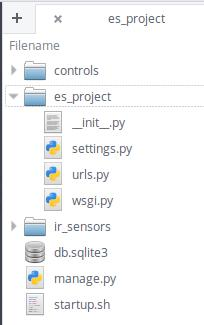
\includegraphics[width=0.3\linewidth]{es_project_directory_1}
%		\caption{}
%		\label{fig:es_project_directory_1}
%	\end{figure}
	
	\begin{figure}
		\hfill
		\subfigure[Main directory \texttt{es\_project/}] {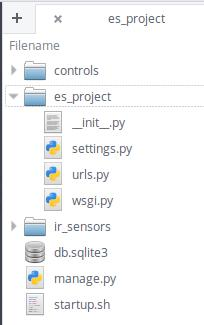
\includegraphics[width=5cm]{es_project_directory_1}}
		\hfill
		\subfigure[Sub directory  \texttt{controls/}]{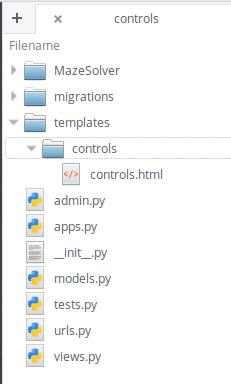
\includegraphics[width=5cm]{es_project_directory_2}}
		\hfill
		\subfigure[Sub directory  \texttt{ir\_sensors/}]{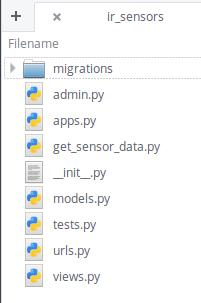
\includegraphics[width=5cm]{es_project_directory_3}}
		\hfill
		\caption{Django project directory layout}
	\end{figure}
	
%	\begin{figure}
%		\centering
%		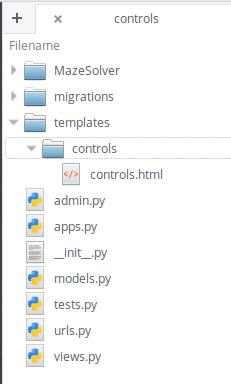
\includegraphics[width=0.3\linewidth]{es_project_directory_2}
%		\caption{}
%		\label{fig:es_project_directory_2}
%	\end{figure}

	
	As a reference, in general the steps outlines in the Django tutorial \cite{DjangoTutorial} should be followed, but some files were modified by us; those changes have been included below.
	
	\begin{description}[font=\quad $\circ$, topsep=-2pt, itemsep=2pt]
		\item \texttt{es\_project/startup.sh}:
		
			% Source: https://www.sharelatex.com/learn/Code_listing
			\lstinputlisting[language=bash]{"./es_project/startup.sh"}
			
			The initial code in this file is used to retrieve the IP address the Pi3 is connected, to using Linux's \texttt{ifconfig} command. We try both \texttt{wlan0} and \texttt{wlan1} (if we had connected an external USB Wifi dongle), and we use whichever is not empty. 
			
			Once we have retrieved this IP address, we use it to start the Django server by executing \texttt{manage.py runserver}. We pass the IP address discovered as an argument.
		
		
		
		\item \texttt{es\_project/es\_project/settings.py}:
		
			% Source: https://www.sharelatex.com/learn/Code_listing
			\lstinputlisting[language=bash]{"./es_project/es_project/settings.py"}
			
			We have modified the code here to add the function \texttt{get\_current\_ip\_address\_str()}, which we use to get the IP address of the connection using the \texttt{pyiface} package and the regular expressions package \texttt{re}. We then add this to \texttt{ALLOWED\_HOSTS} in the next line.
		
		
	\end{description}
